\section{Suggestive Interface for Shape Modification }\label{sec:interaction}
%
For some creative designs, the rough 3D carton model generated based on our heuristic approach still needs some improvements or the user might edit the carton shape. 
%After folding the flat layout into a rough shape, we need to refine the model to final state through basic geometric constraints and user-selected constraints which are obtained from user interaction. 
To assist users to refine the carton model, our system is equipped with a set of smart shape refinement operations, such as automatically detecting vertexes that can be merged, propagating modification to similar groups, and providing suggestions for users to explore. 
%
While a user edits the carton model in the 3D space, which is more intuitive, our system is capable of revising the 2D layout automatically. 

%Figure~\ref{fig:interface} illustrates two operations that the system provides, the first one is selecting points need to be merged by users and the second is select the right option from results by vertex merging detection.   

%\begin{figure}
%	\centering
%	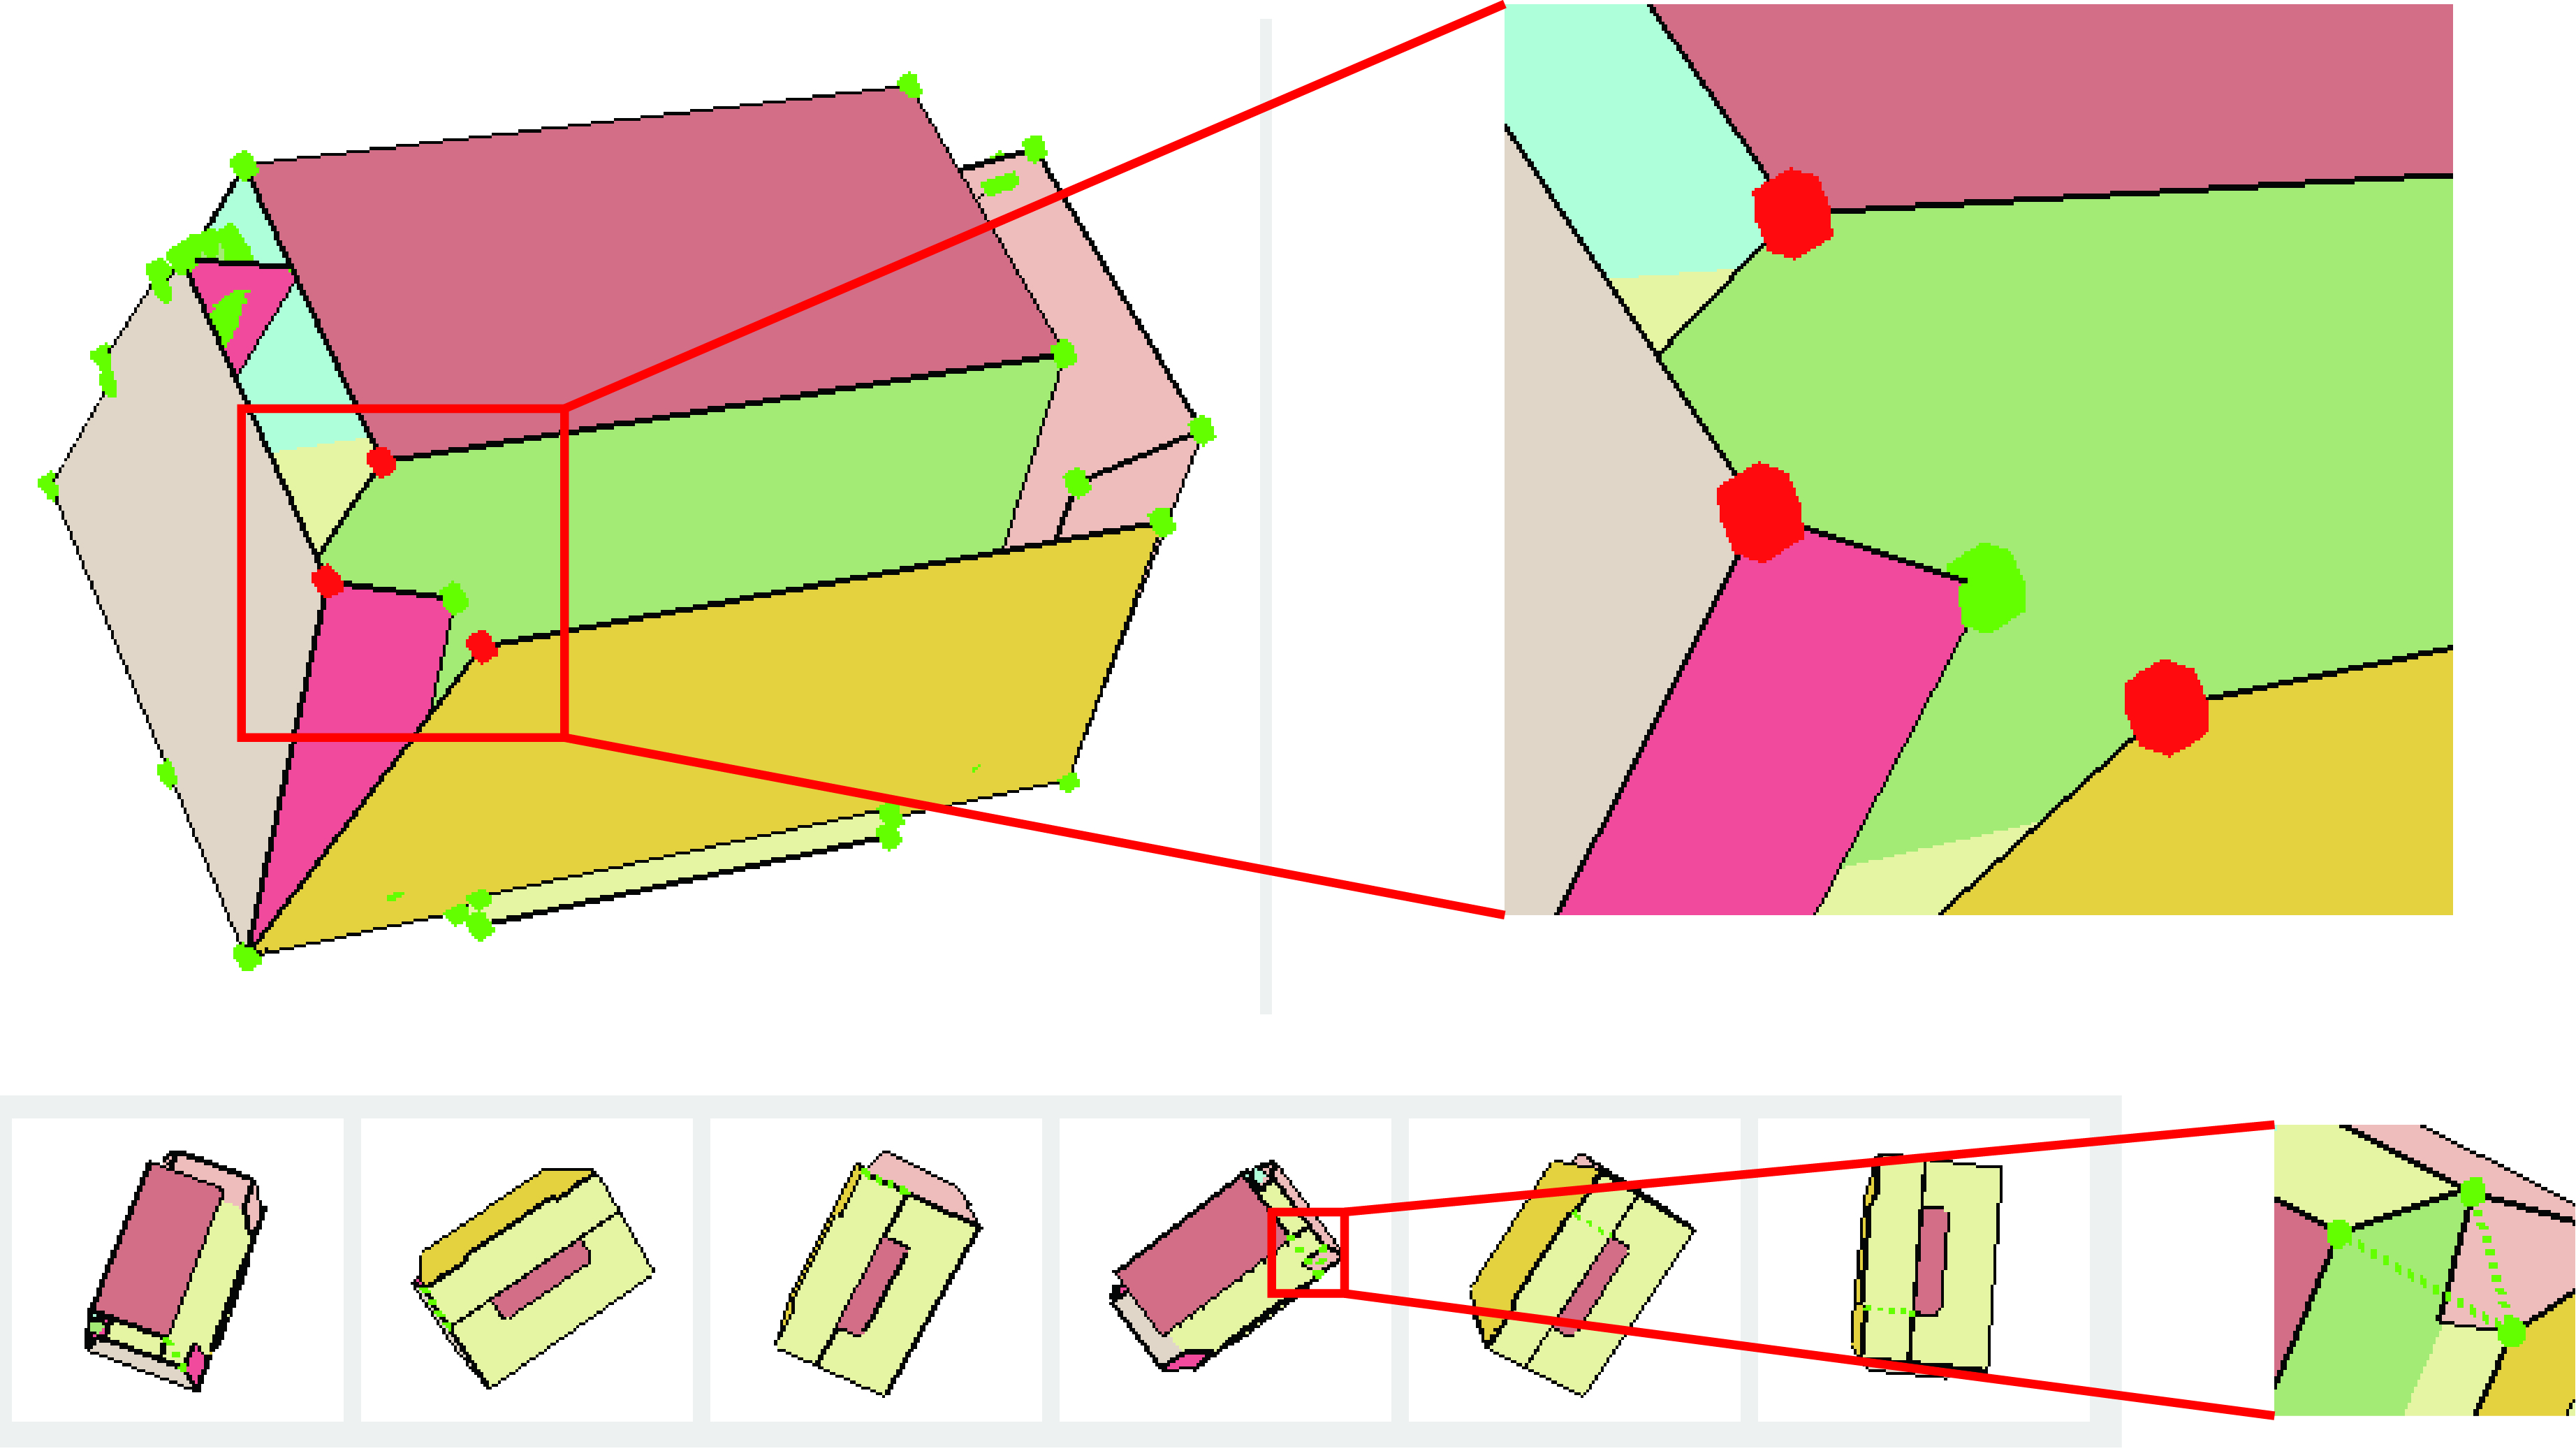
\includegraphics[width=0.9\textwidth]{images/UIdetail.jpg}
%	\caption{two operations that the system provides}
%	\label{fig:interface}
%\end{figure}

\subsection{Suggestive Interaction}

Our system automatically detects a group of potential shape constraints to improve the 3D carton model.
%
These guiding constraints are provided to the user for quickly selecting and manipulating the carton shape.
In our system, three types of shape refinement operations, vertex merging, merging propagation, and face pasting, are automatically detected.

%
%In order to assist users construct the final carton interactively, we also provide symmetry detection and merging points detection to improve the efficiency of constructing models .

\paragraph{Vertex Merging.} 
For irregular shapes which consist of non-rectangular panels or non-perpendicular adjacent panels, some vertexes are close to each other after the initialization step.
A practical carton model can be obtained by simply merging these nearby vertexes together if their have coherent edges.
%
Any pair of vertexes $\mathbf{v}_a$, $\mathbf{v}_b$ in different panels is detected as mergeable, if $|\mathbf{v}_a-\mathbf{v}_b|<\epsilon$, and there is an edge connecting to $\mathbf{v}_a$ having the equal length with one edge connecting to $\mathbf{v}_b$,
%
$\epsilon$ is a distance threshold and set as 50mm in our experiments.
More vertexes can be merged together, as shown in Figure~\ref{fig:suggestion:a} by gradually adding one vertex $\mathbf{v}$ each time if $\mathbf{v}$ is mergeable with at least one vertex in current list. 
%Consider the initialization results can represent the ideal model partly, the disadjacent vertices that have one edge with same length can be regarded as targets that need to be located in the same place if their Euclidean distance is below a certain threshold.

\paragraph{Merging Propagation.} %{\color{blue}{focus on the symmetry property of vertexes.
Once the user makes a decision to merge a subset of vertexes $\mathbb{V}=\{\mathbf{v}_i\}_{i=1,\ldots,K}$ from automatic system suggestions or manually selection, our system will detect if there exists another subset of vertexes $\vset_b$ symmetric to $\mathbb{V}$ and propagate the merging operation to $\vset_b$, as shown in Figure~\ref{fig:suggestion:b}. 
A subset $\mathbb{V}_b$ is symmetric to $\mathbb{V}_a$ if $|\vset_a|=|\vset_b|$, and there exists one-to-one correspondence between the vertexes in $\vset_a$ and $\vset_b$. 
Here, $|\vset|$ is the number of vertexes in a vertex subset $\vset$. 
Two vertexes $\vn_a$ and $\vn_b$ are defined as corresponding vertexes if they have the same number of edges and one-to-one correspondence can be found between the edge lengths. 

\begin{figure}
	\centering
	 \subfigure[Vertex merging]{
	 	\label{fig:suggestion:a} %% label for first subfigure
	 	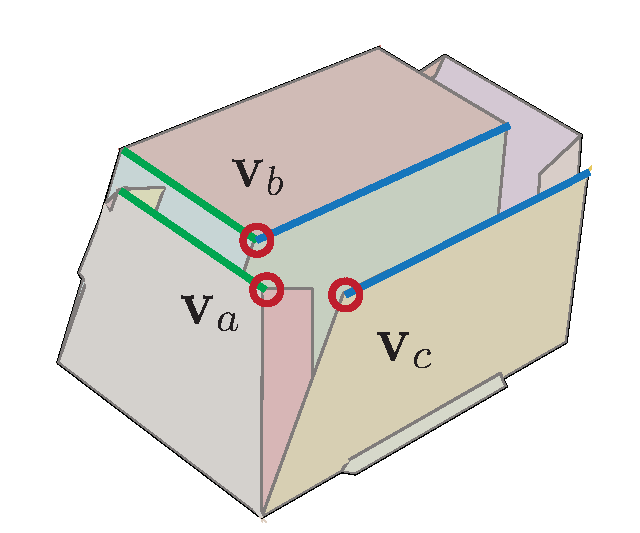
\includegraphics[width=0.3\textwidth]{images/suggestiona.pdf}}
	 \hfill
	 \subfigure[Merging propagation]{
	 	\label{fig:suggestion:b} %% label for second subfigure
	 	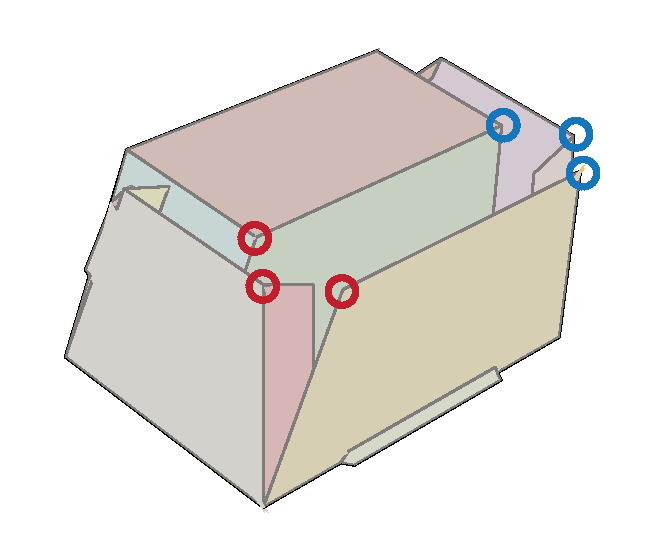
\includegraphics[width=0.3\textwidth]{images/suggestionb.pdf}}
	 \hfill
	 \subfigure[{Panel pasting}]{
	 	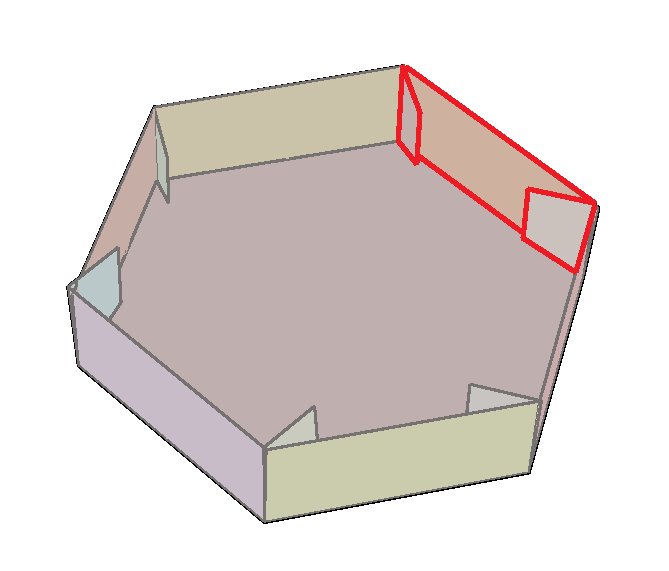
\includegraphics[width=0.3\textwidth]{images/suggestionc.pdf}
	 	\label{fig:facepasting}
	 	}
	 
	 \caption{Three different suggestions on shape modification. (a) A group of vertexes (marked in red) are detected as mergeable. $\mathbf{v}_a$ and $\mathbf{v}_b$ are close to each other and one edge connecting to $\mathbf{v}_a$ has the same length with one edge connecting to $\mathbf{v}_b$ (green edges). $\mathbf{v}_c$ is also considered to be merged with $\mathbf{v}_a$ and $\mathbf{v}_b$ because $\mathbf{v}_c$ is close to $\mathbf{v}_b$ and one edge of $\mathbf{v}_c$ has the same length as $\mathbf{v}_b$ (blue edges). (b) Once the user confirms a suggested vertex merging operation, our system automatically proposes a symmetric group of vertexes that can be also merged (marked in blue). (c) If the panels marked in red are detected close to each other and the same with their normals, our system suggests these panels can be sticked together.}
	 \label{fig:suggestion}
\end{figure}

%\begin{figure}
%	\centering
%	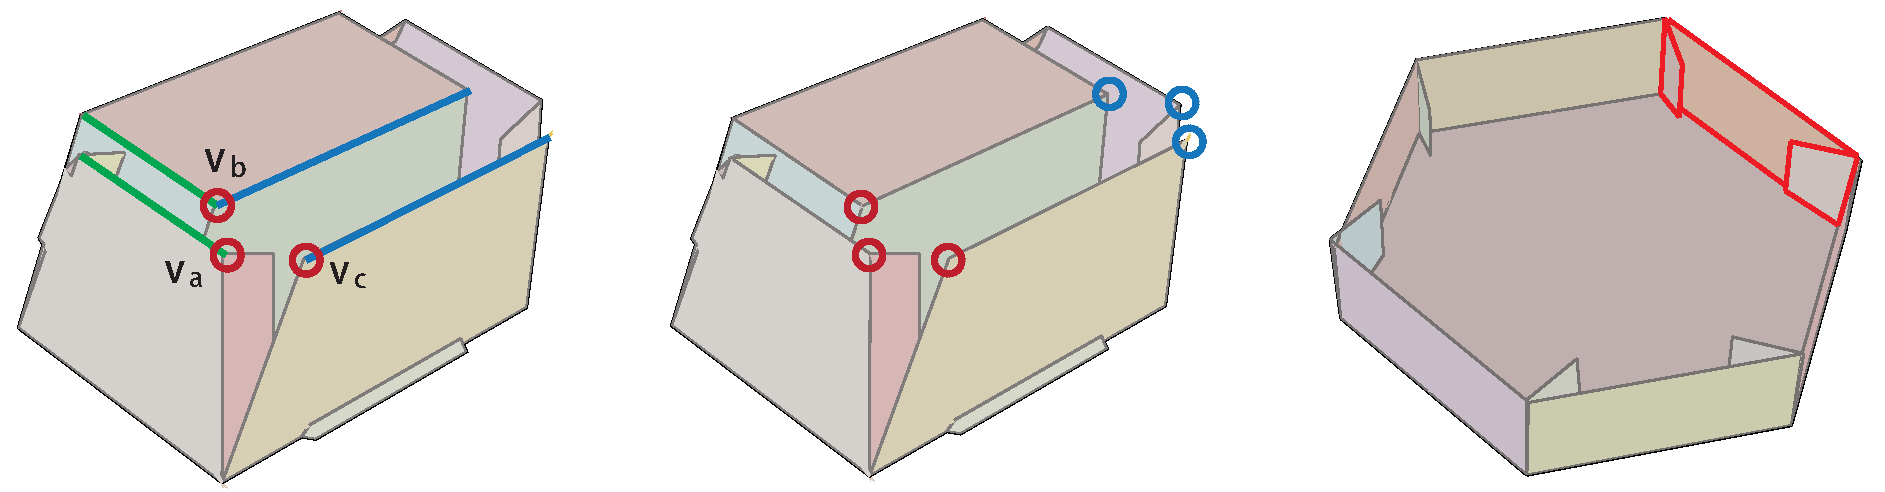
\includegraphics[width=0.9\textwidth]{images/suggestion}
%	\caption{Vertex merging detection is well illustrated by (a), $\mathbf{v}_a$ and $\mathbf{v}_b$ may have the need to merge cause $|\mathbf{v}_a-\mathbf{v}_b|<\epsilon$, and one edge connecting to $\mathbf{v}_a$ marked as green has the same length with one edge connecting to $\mathbf{v}_b$ also marked as green. $\mathbf{v}_c$ can also be considered that need to merge with $\mathbf{v}_a$ and $\mathbf{v}_b$ as $|\mathbf{v}_c-\mathbf{v}_a(\mathbf{v}_b)|<\epsilon$ and one of incident edges of $\mathbf{v}_c$ marked as blue has the same length as $\mathbf{v}_a(\mathbf{v}_b)$'s also marked as blue. While users select three vertexes circled in red (b), our system can detect symmetric vertexes circled in blue automatically. \cxj{show more possible suggestions in this figure. Make sure the font in consistent with the caption}.\cxj{use subfigure?}}
%	\label{fig:suggestion}
%\end{figure}

\comments{
	$\mathbf{v}_a$ and $\mathbf{v}_b$ are regarded as symmetric pair, if for each pair of $l_{ai} \in \{ l_{a1},l_{a2}...l_{am}\}$ and $l_{bi} \in \{ l_{b1},l_{b2}...l_{bn}\}$, $m = n$ and $|l_{ai}- l_{bi}|<\epsilon$ where $m$ is the number of $\mathbf{v}_a$'s ordered set of the incident edges' length $\{ l_{a1},l_{a2}...l_{am}\}$, and $n$ is the number of $\mathbf{v}_b$'s ordered set of the incident edges' length $\{ l_{b1},l_{b2}...l_{bn}\}$.
	
	When involving multiple vertexes, the searching criterion is based on symmetric vertex pair detection described above. The symmetric vertex set of selected vertexes $\{\mathbf{v}_1,\mathbf{v}_2,...,\mathbf{v}_{n-1}\}$ is $\{\hat{\mathbf{v}}_1,\hat{\mathbf{v}}_2,...,\hat{\mathbf{v}}_{n-1} \}$, the vertex set $\{\mathbf{v}_1,\mathbf{v}_2,...,\mathbf{v}_n\}$ has the symmetric vertex set $\{\hat{\mathbf{v}}_1,\hat{\mathbf{v}}_2,...,\hat{\mathbf{v}}_n \}$, if $||\mathbf{v}_n-\mathbf{v}_i| - |\hat{\mathbf{v}}_n-\hat{\mathbf{v}_i}||<\epsilon$, for $i = 1,....,n-1$.
}

\comments{Take Figure~\ref{fig:suggestion} (b) as an example, after users selecting vertexes circled in red, our system can automatically detect their symmetric set circled in blue. As an result, our system can detect these symmetry pairs to assist users improve efficiency.}

\paragraph{Panel Pasting.} Merging vertexes sometimes is not enough to generate desired model caused by the glue flap as shown in Figure~\ref{fig:facepasting}. A pair of panels $P_a$ and $P_b$ is considered mergeable if their normals $\mathbf{n}_a$ and $\mathbf{n}_b$ satisfy $\mathbf{n}_a \cdot \mathbf{n}_b > 0.5$, and for each vertex in $\{\mathbf{v}_{ai}\}_{i=1}^{N_a}$,  $|(\mathbf{v}_{ai} - \mathbf{v}_{c}^b) \cdot \mathbf{n}_b| < \epsilon_d$, where $\mathbf{v}_{c}^b$ is the centroid of the panel $P_b$, and $\mathbf{n}_b$ is the normal. When involving multiple panels, the detection strategy is the same with our vertex merging. 



\comments{
\begin{figure}
	\centering
	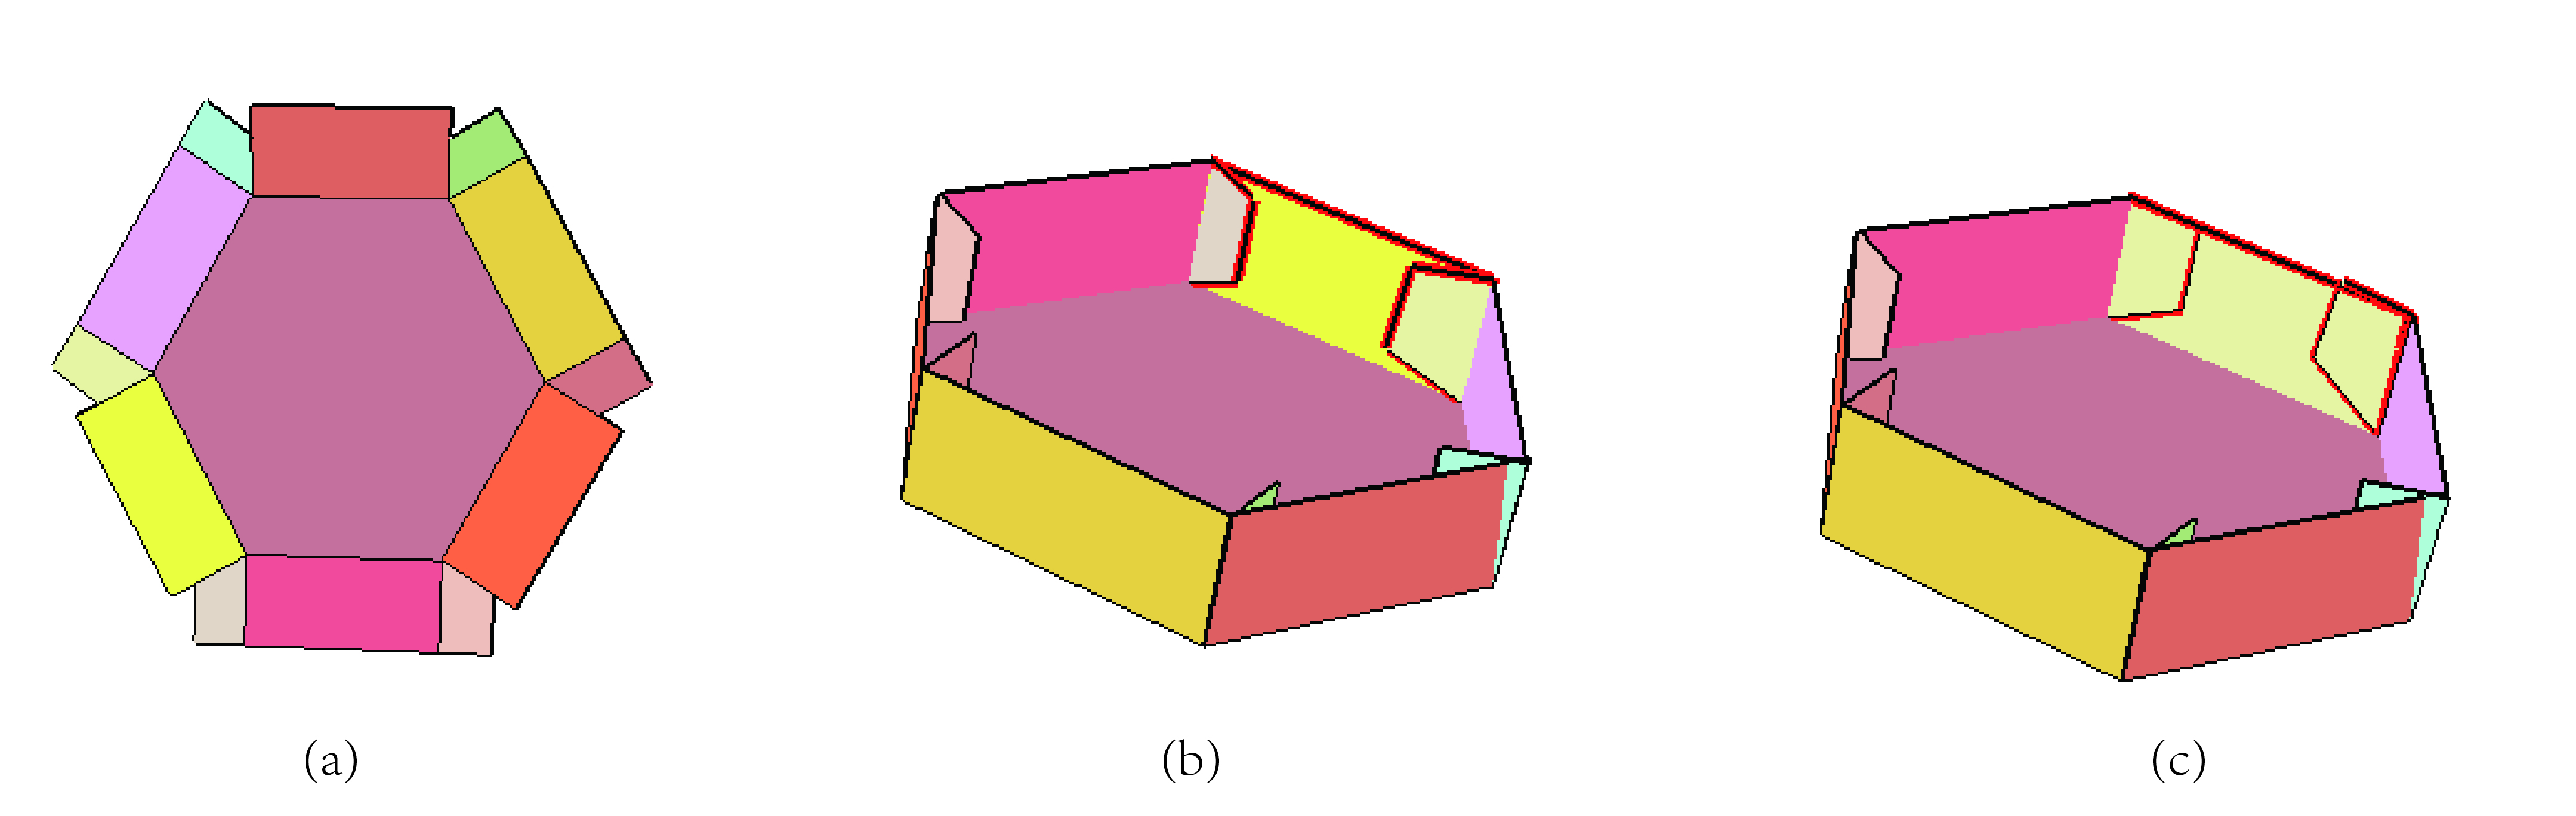
\includegraphics[width=0.9\textwidth]{images/facepaste.jpg}
	\caption{The initialization result (b) of hexagonal box layout (a) can not reach an ideal state by merging vertexes, hence our system allow users to select merging panels which are bounded by red lines (b) and enforce planarity to the model, the result is shown by assigning same color to the coplane panels (c).}
	\label{fig:facepaste}
\end{figure}

\begin{figure}
	\centering
	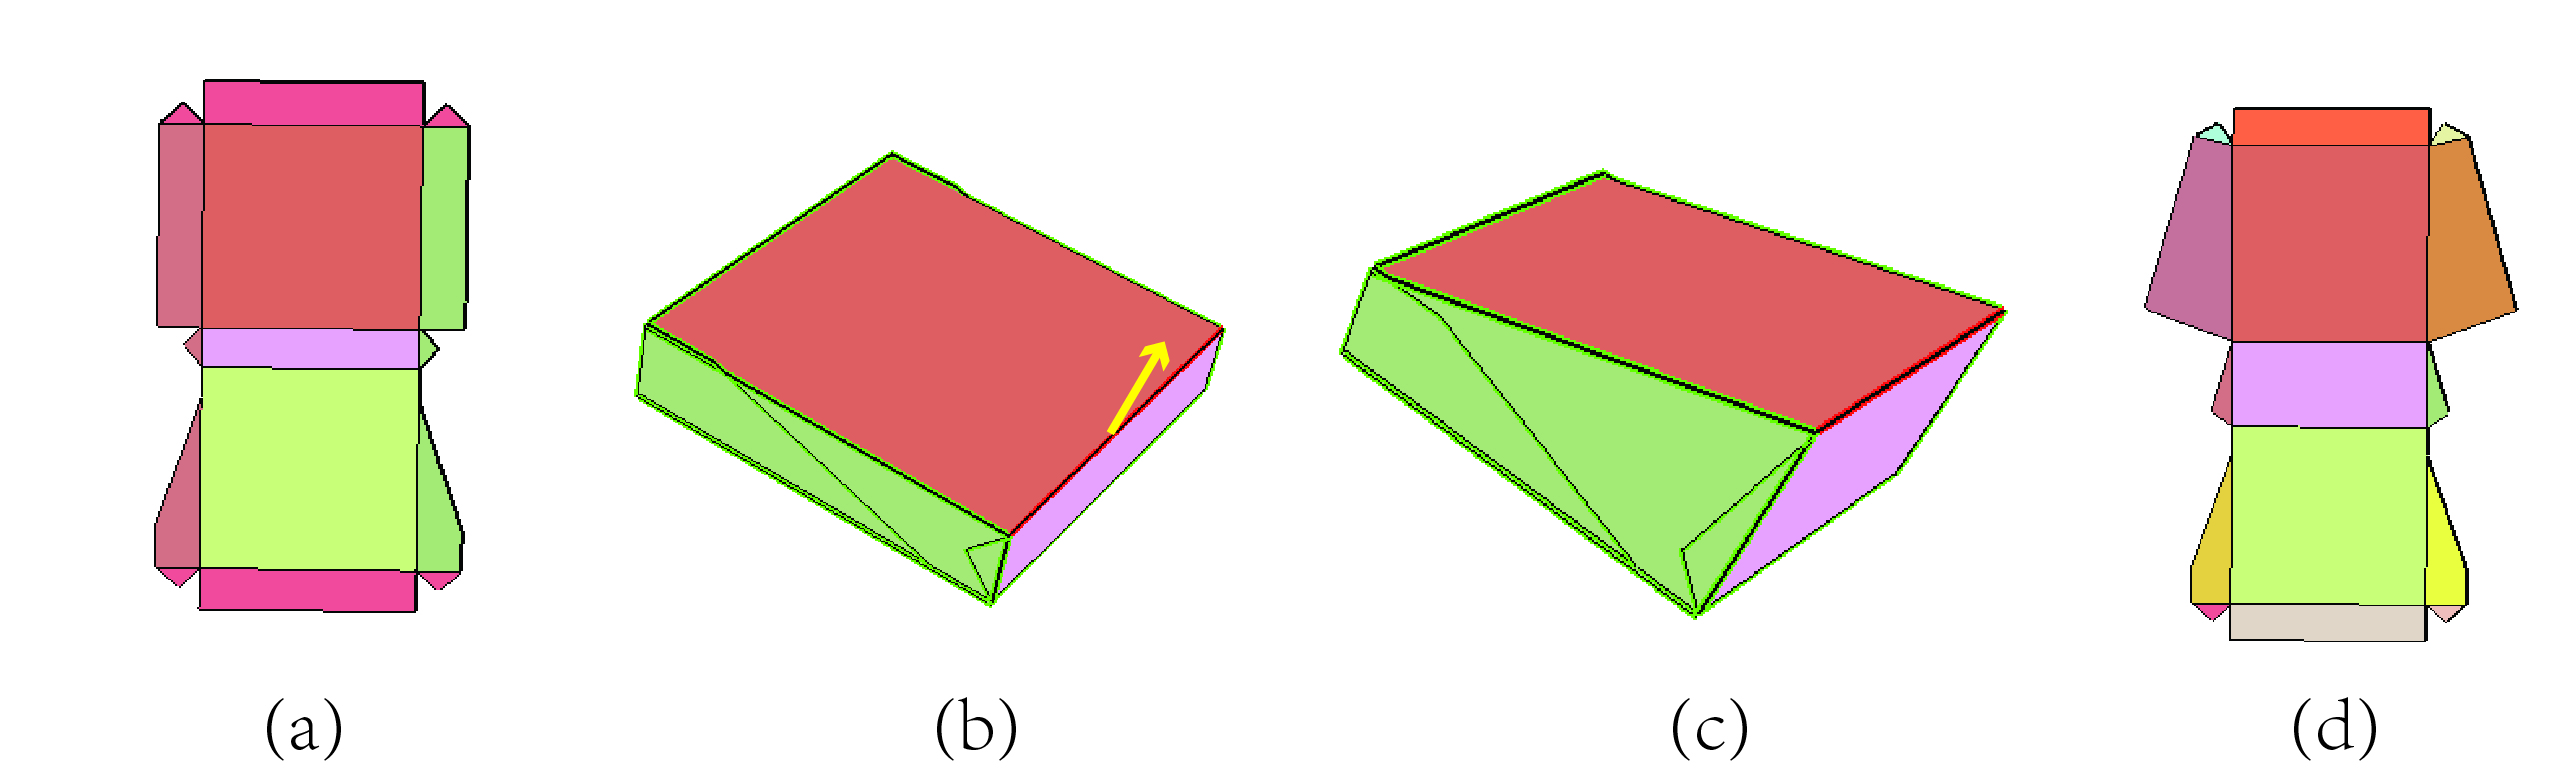
\includegraphics[width=0.9\textwidth]{images/editing.jpg}
	\caption{A standard cuboid carton (b) can be generated by the layout (a). Users are allowed to edit the shape of 3D model by dragging the edges, then the model will be deformed to a novel carton (c), by enforce the constrains to layout, our system can generate a deformable layout automatically as (d) shows.}

\end{figure}
}


\subsection{2D Layout Refinement from 3D Editing}

While it is significantly efficient to generate a 3D carton using our approach from an existing 2D layout, our system allows users to creatively edit the current 3D carton model by dragging an edge and simultaneously refines the 2D layout automatically according to the 3D editing.
%
When the 3D mesh changes, the new shape constraints are transferred to the 2D layouts by keeping panel rigidity (Eq.~\ref{equ:plane}).
Since the layout remains in a 2D plane, the coplanarity is enforced for all the vertexes in the layout. 
%
% 
The irrelevant vertexes that do not lie on the moving edge have to stay at their original locations, as described in Eq.~\ref{equ:irrelevant}.
Figure~\ref{fig:editing} shows two examples of automatic layout refinement from 3D editing.                                                                     

\begin{figure}
	\centering
	\subfigure[]{
		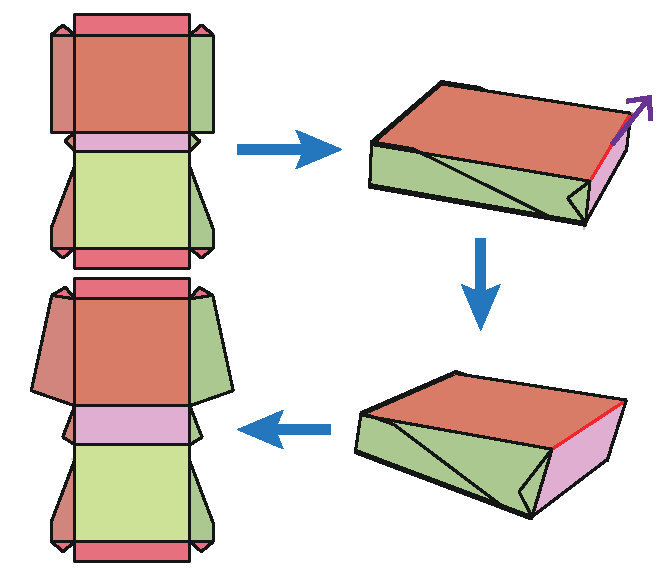
\includegraphics[width=0.4\textwidth]{images/editing1}
		\label{fig:editing1}
	}
	\hspace{4ex}
	\subfigure[]{
		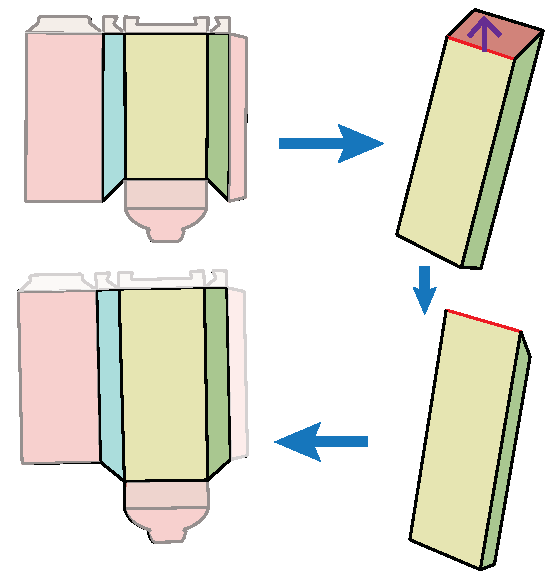
\includegraphics[width=0.35\textwidth]{images/editing2}
		\label{fig:editing2}
	}
	\caption{Two examples of layout modification from 3D model editing. For each example, a box-like carton can be generated from the given 2D layout. Users can edit the shape of the 3D carton by dragging edges in our system. By enforce the shape rigidity constrains, our system automatically updates the 2D layout.}
	\label{fig:editing}
\end{figure}


